% Asset ID: AS1StraightLineGraphsTikZ-001
% Source: P1-Chp5-StraightLineGraphs_RevealBlocksRemoved.pdf; transcript; CCEA specification map
% Related lesson section: Core Theory, Section 3: Gradient
% Purpose: Show a gradient triangle labelled Delta x, Delta y, and m = Delta y / Delta x.

\documentclass[tikz,border=8pt]{standalone}
\usepackage{amsmath}
\usepackage{tikz}
\usetikzlibrary{arrows.meta,calc,positioning}

\begin{document}
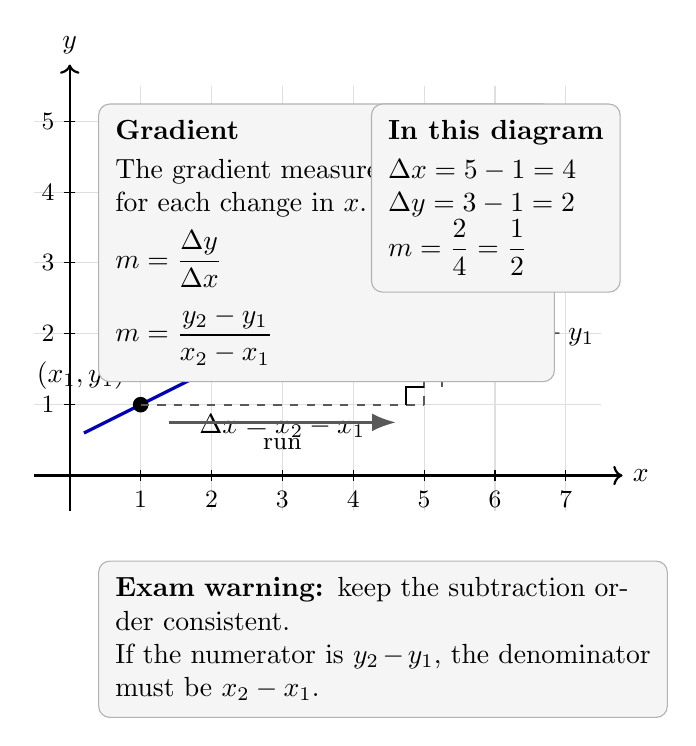
\begin{tikzpicture}[
    scale=0.9,
    axis/.style={->, thick},
    gridline/.style={gray!25, thin},
    mainline/.style={very thick, blue!70!black},
    helper/.style={thick, dashed, gray!70!black},
    point/.style={circle, fill=black, inner sep=2pt},
    labelbox/.style={draw=gray!60, rounded corners, fill=gray!8, inner sep=6pt, align=left}
]
\draw[gridline] (-0.5,-0.5) grid (7.5,5.5);
\draw[axis] (-0.5,0) -- (7.8,0) node[right] {$x$};
\draw[axis] (0,-0.5) -- (0,5.8) node[above] {$y$};
\foreach \x in {1,2,3,4,5,6,7}{\draw (\x,0.08) -- (\x,-0.08); \node[below] at (\x,-0.08) {\small \x};}
\foreach \y in {1,2,3,4,5}{\draw (0.08,\y) -- (-0.08,\y); \node[left] at (-0.08,\y) {\small \y};}
\coordinate (A) at (1,1);
\coordinate (B) at (5,3);
\coordinate (C) at (5,1);
\draw[mainline] (0.2,0.6) -- (7.2,4.1) node[pos=0.88, above, sloped] {straight line};
\node[point, label=above left:{$(x_1,y_1)$}] at (A) {};
\node[point, label=above right:{$(x_2,y_2)$}] at (B) {};
\draw[helper] (A) -- (C);
\draw[helper] (C) -- (B);
\draw[thick] ($(C)+(-0.25,0)$) -- ($(C)+(-0.25,0.25)$) -- ($(C)+(0,0.25)$);
\node[below] at ($(A)!0.5!(C)$) {$\Delta x=x_2-x_1$};
\node[right] at ($(C)!0.5!(B)$) {$\Delta y=y_2-y_1$};
\draw[-{Latex[length=3mm]}, thick, gray!70!black] (1.4,0.75) -- (4.6,0.75);
\node[below] at (3,0.65) {\small run};
\draw[-{Latex[length=3mm]}, thick, gray!70!black] (5.25,1.25) -- (5.25,2.75);
\node[right] at (5.35,2) {\small rise};
\node[labelbox, anchor=north west] at (0.4,5.25) {\textbf{Gradient}\\[2pt]
The gradient measures change in $y$\\
for each change in $x$.\\[4pt]
$\displaystyle m=\frac{\Delta y}{\Delta x}$\\[6pt]
$\displaystyle m=\frac{y_2-y_1}{x_2-x_1}$};
\node[labelbox, anchor=north west] at (4.25,5.25) {\textbf{In this diagram}\\[2pt]
$\Delta x=5-1=4$\\
$\Delta y=3-1=2$\\
$\displaystyle m=\frac{2}{4}=\frac12$};
\node[labelbox, anchor=north west, text width=6.8cm] at (0.4,-1.2) {\textbf{Exam warning:} keep the subtraction order consistent.\\
If the numerator is $y_2-y_1$, the denominator must be $x_2-x_1$.};
\end{tikzpicture}
\end{document}
